\RestyleAlgo{boxed}
\chapter{并行层次概率计算模型}
\section{引言}
在本章中,我们将这个目标词表示扩展到一个分层的形式,使它们适配基于类的分层概率计算。首先,我们提出了一个在分层结构上建模参数的字编码方案。因此,考虑到GPU上的并行吞吐性能,我们推导出紧凑的代价函数及其梯度。

同时,类上的单词分布对其性能有很大的影响,应该在训练阶段之前定义,我们在本次实验中并不考虑那些在训练过程中动态交换算法,即一边训练模型一边动态改变了单词群结构。我们采用了几个词汇分割策略,基于单词或者文本的统计、句法和语义知识来初始化其结构,以达到一个稳定和可以预期的性能。

而且,在推理过程中,不同于传统的softmax情况,得到最好的候选者自然是可行的,层次推理不能直接用 softmax 方法来实现。我们讨论基于类的搜索策略的两种不同的推理情况:a)打分:输出给定序列的概率;b)排序   :在给定的上下文中获取得分最高的一个候选单词。

\begin{table}[!ht]
  \centering
  \caption{并行层次概率计算模型的符号助记表}
\begin{tabular}{llc}
  \toprule
   符号&涵义&取值范围\\ \midrule
$\theta^c\in\mathbb{R}^m$ &表示单词的类别向量& Float32\\
$ \theta^o$ &表示路径$l^w$表示划分后的单词三维张量&Float32 \\
$\Gamma'$ &路径查找表,给定单词元祖序列,可以获得对应的单词& \\
  \bottomrule
\end{tabular}
\end{table}
\section{词表划分编码}
为了提高GPU架构的加速比,并支持广义的词汇分割方法,我们提出了一种基于类的分层softmax方法的高效通用结构。

扁平化的词汇表被分成类别向量$ \theta^c $和输出矩阵$ \theta^o $ 结构,其中前者定义了不同类别的概率$ p ^ c $,而后者则模拟了该分区组内的单词概率$ p ^ o $,如图~\ref {fig:chsm}~所示。输出矩阵的维度是:类维度和分组词维度。如果将词汇$ \mathcal {V} $划分为不等大小的组,我们首先将词组分类为等长矩阵,填充零掩码。对于不在这个组中的剩余节点,我们使用掩码向量$ \theta ^ m $来消除其对概率计算和成本汇总过程的影响。因此,分组的文字长度是最大的组长度。如果我们应用相同大小的词汇分割算法,掩码向量则~$\theta^m$~可以被忽略,并且分组的词维度是$ \mathcal {| V | / | C |} $,其中$ \mathcal {| C |} $表示类维度。这里我们需要注意的是,如果$ \mathcal {| V |} $不能被$ \mathcal {| C |} $整除,那么最后一组中的实际的单词数量应该小于该组的大小。但我们并不打算采用特殊的结构来处理这个问题。因为尽管这些不存在的单词会稀释该组中其他单词的概率大小。但是一方面不影响其他类别的概率计算,另一方面也不影响该组中,其他单词的概率顺序关系。因此实际影响比较小。
\begin{figure}[!ht]
  \centering
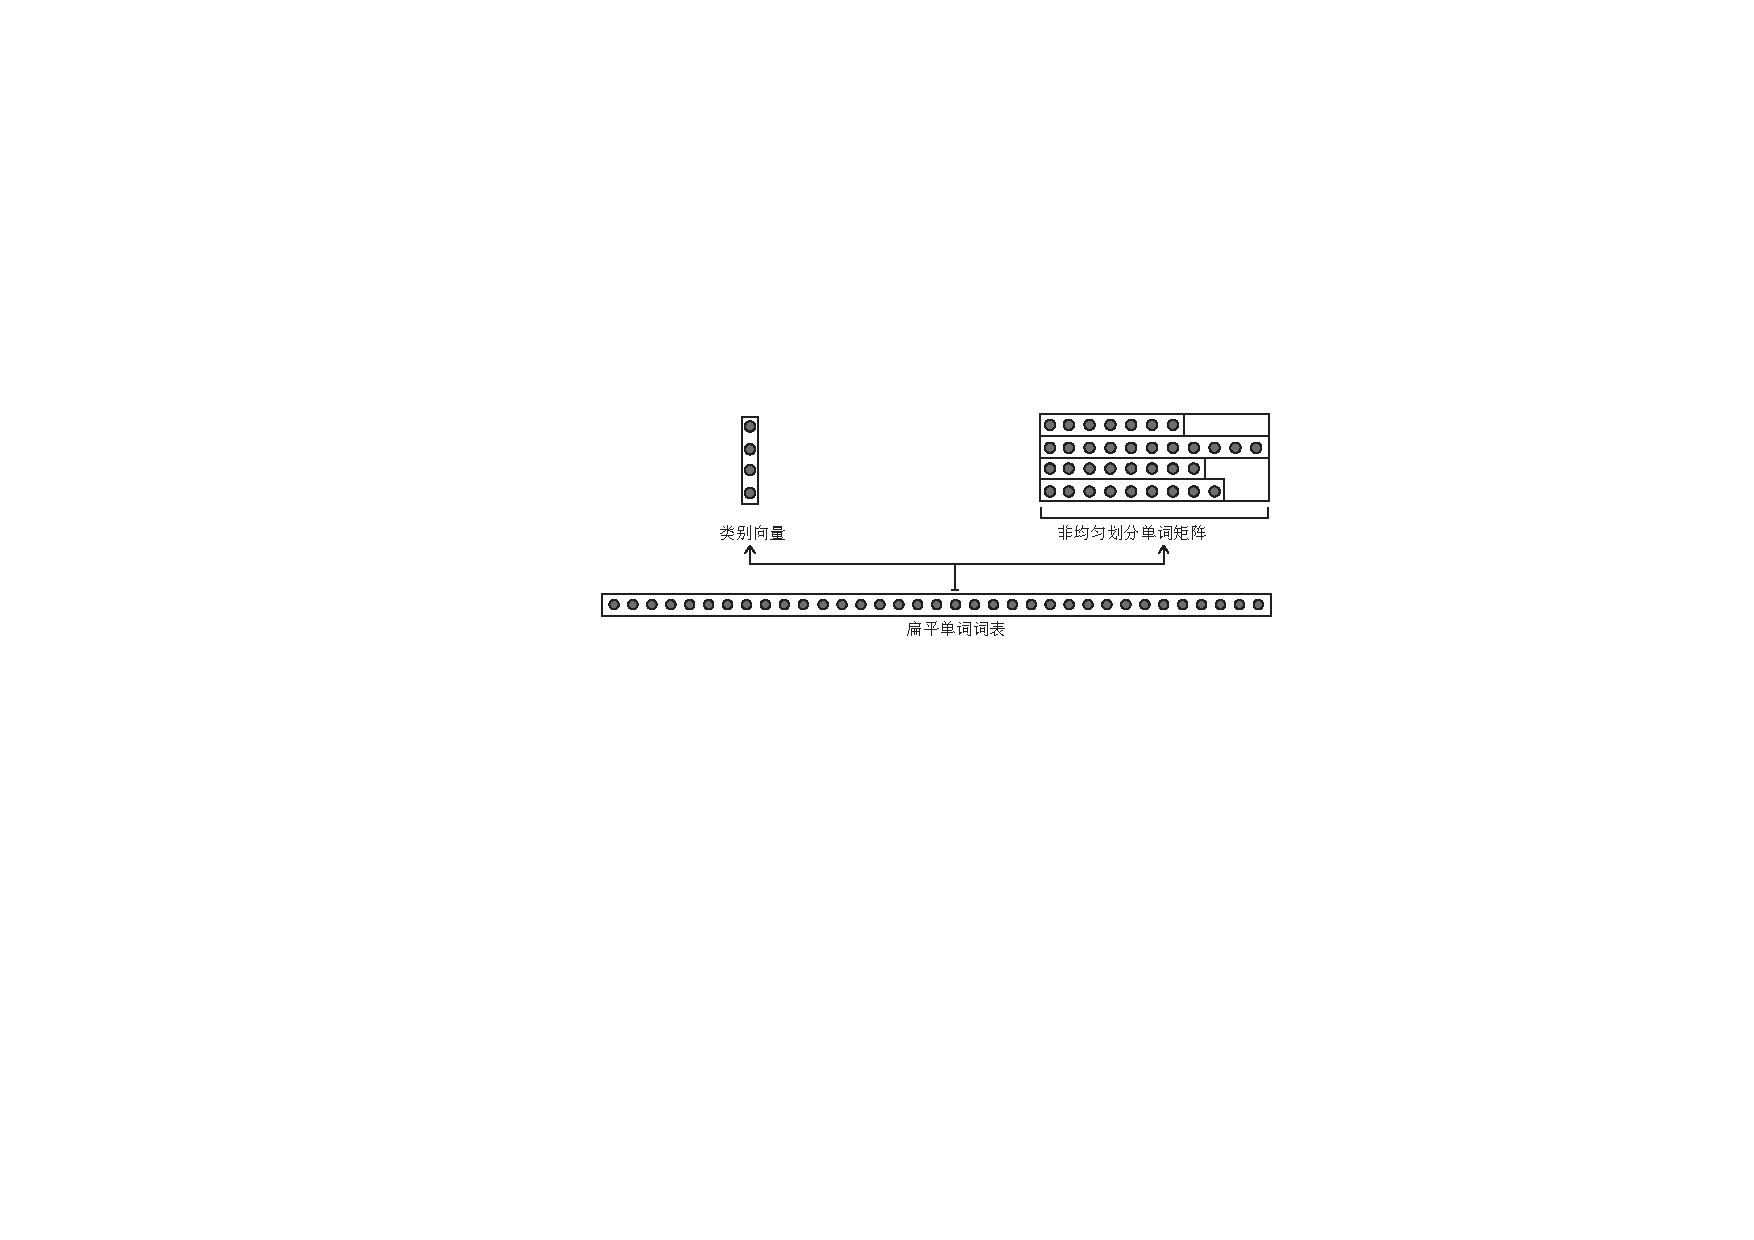
\includegraphics[width=0.85\linewidth]{./figures/chsm-simple.pdf}
\caption{cHSM算法的两种不同的词表划分算法}\label{fig:chsm}
\end{figure}


更重要的是,我们将一维的单词索引替换成一个元组单词索引$(w ^ c,w ^ o)$,可以利用该元组从我们预先定预先定义的查找表$\Gamma $中检索给定单词索引$ w $。此外,$ w ^ c $指代的是单词的类别编号,$ w^c $表示该组内的本地单词索引。
\begin{equation}\label{equ:partition}
 \theta^m=
\begin{cases}
    \text{单位矩阵} ,& \text{若均匀划分} \\
    \text{掩码矩阵},   & \text{否则}
\end{cases}
\end{equation}


如图~\ref{fig:chsm}~所示,扁平化的词汇可以形成右上矩阵,矩阵的大小应该大于或等于词汇表,不需要外部掩码。
另外,拼合词汇可以形成左上矩阵,需要外部掩码,矩阵的分布算法依赖于具体的词表分割算法。

\section{基于类别的代价函数和导数}
当我们定义了单词基于类别的二元编码后,我们接下来讨论基于这种编码的代价函数和导数计算公式。
给定最后一个隐藏层输出$ h $,那么这个分区组中的每个组和每个单词的概率可以被定义为:
\begin{equation}
\begin{split}
\log p^c(c|h) &= \theta^c h-\log \sum{\exp( \theta^c h )} \\
\log p^o(w|w^c,h)&=\theta^o h -\log\sum\exp{(\theta^o h)}
\end{split}
\end{equation}
其中$ p ^ c $和$ p ^o $是分别计算而不是并行计算的,因为主要的计算瓶颈是局部标准化的单词概率$ p ^ o $,所以这两个概率的并行计算不会达到时间效率提升。

\subsection{概率稀释问题}
尽管如此,掩码矩阵不能直接应用于这个分词矩阵,应该应用在对数概率归一化(log softmax)的计算程序中。 为了说明,在softmax函数中:$ p(x_i)= {\exp({x_i}})/ {\sum_j \exp(x_j)} $,如果$ x_k = 0 $,但其概率$ p(x_k)> 0$因为$\exp(x_k)> 0 $。即:对于不存在的类别中的单词,我们仍然有概率分布,这样对于那些实际存在的单词概率来说,至多有$\mathcal{|V|/\mathcal{C}}-1$的类别存在这样的概率稀释问题。

 因此,该组中确切的后验词对数概率计算如下:
\begin{equation}
  \log p^o(w|w^c,h)=\theta^o h -\log\sum\theta^m\exp(\theta^o h)
\end{equation}

那么,这个模型的损失函数可以形式化地定义成如下形式:
\begin{equation}
\ell(\theta|h) =\log p^c(w^c|h) +\log p^o(w^o|w^c,h)
\end{equation}
其中在类别层次损失等于负对数似然函数(代价函数),并且单词级别的损失需要在计算其损失时指定其类别 $ w ^ c $。

在训练过程中,$ w ^ c $是需要预先定义的的,然而在测试过程中,$w^c$需要预先计算最有可能的类别,即由公式$\tilde w^c=\arg\max_c p^c$计算获得获取。 

类似地,模型的所有的参数$\{\theta^c,\theta^o,h\}$对于模型的代价函数的导数计算公式如下:
\begin{equation}
\begin{split}
\frac{\partial \ell}{\partial \theta^c}=& (\delta_{ij}-p(c|h))h \\
\frac{\partial \ell}{\partial \theta^o}=&(\delta_{ij}-p(w|c,h))h \\
\frac{\partial \ell}{\partial h}=&(\delta_{ij}-p^c(c|h))\theta^c + (\delta_{ij}-p^o(w|c,h))\theta^o
\end{split}
\end{equation}

将词汇分成相互排斥的词组的一个主要优点是:a)避免了在整个词汇表上归一化概率。 由于$ p ^ c $是在类维度上概率归一化(Normalization)的,$ p ^ o $是在最大组大小维度上进行概率归一化的。 所以在第二个方程中,多余的其他组被忽略,在最大的文本数据集中二者都不会超过1000。 b)与基于树的结构相比,它在词汇表上的结构性约束(Structural Constraint)更少,在分解步骤中丢失的信息更少。 c)与子字级方法相比,它不会增加序列长度,也不会影响循环神经网络的长程依赖建模问题。



\section{基于类别的测试推理}
在推理阶段,对于cHSM模型来说,序列的概率评分要容易得多。
类似于以前的方法,我们可以通过重新研究我们的训练模型来解决第一个问题:
\begin{equation}\label{equ:class_inf}
   \log p(w_1,\cdots, w_T)=\sum_t^T\log p(w_t|h_t)=\sum_{t=1}^{T}\log p^c(w^c_t|h_t) +\log p^o(w^o_t|w^c_t,h_t)
\end{equation}
我们发现这种类型的操作比传统的softmax方法有效得多,该方法涉及$ \mathcal{O(|H|\sqrt{|\mathcal{V}|})}$计算复杂度。

\begin{algorithm}[!ht]
\caption{基于 cHSM 算法的全局 $\arg\max$ 算法}\label{alog:alls}
\KwData{ 隐藏层输出 $h$}
 \For{$c \in \mathcal{C}$ }{
  {Calculate $\log p^c(c|h)$} \tcp*[r]{计算类别的概率}
 \For{w $\in$ c}{
 {Calculate $\log p^o(\hat w^o|\hat y^c,h)$} \tcp*[r]{计算单词的条件概率}
  {$\log p(w|h)=\log p^c(w^c|h)+\log p^o(\hat w^o|\hat w^c,h)$}\tcp*[r]{计算每个单词全局概率}
 }
 }
 {$w=\arg\max_w \log p(w|h)$}\;
 \KwResult{概率最大的候选单词$w$。}
\end{algorithm}

其次,对于$\arg\max $的情况,我们可以在选择最佳候选项之前计算词汇表中所有单词的概率,这在直观上是正确的,但在
,因为涉及到整个单词的分割矩阵。 此外,我们仍然可以在算法~\ref{alog:exact}~中对上述方法进行少量修改,然后计算确切的最高候选人。
\begin{algorithm}[!ht]
\caption{基于 cHSM 算法的正确 $\arg\max$ 算法}\label{alog:exact}
\KwData{ 隐藏层输出 $h$}
 {$\hat w^o=\arg\max_o{\log p^o(w| c,h)}$ }\tcp*[r]{挑选每个类中概率最大的类别}
 {// 在这些已经被栅选单词中挑选最佳的单词}
 {$\tilde w^c=\arg\max_c{\log p^c(w^c|h)+\log p^o(\hat w^o|\hat y^c,h)}$}\;
通过查找表 $\Gamma'$ 将 $(\tilde w^c,\hat w^o[\tilde w^c])$替换成单词$w$ \;
 \KwResult{概率最大的候选单词$w$。}
\end{algorithm}

\subsection{标签偏差问题}
此外,cHSM算法的性能对词表划分算法有些敏感,因为某些方法可能会产生高度不平衡的字组,并且这种单词不均匀分布会在算法中产生标签偏差问题(Label Bias)。第一个本地 $\arg\max_o$ 进程~\upcite{DBLP:conf/icml/LaffertyMP01}。然而,在大多数情况下,如果选择合适的参数,则可以考虑不平衡的问题,本文考虑平衡词汇分区的广义形式。

我们接下来来详细说明标签偏差问题。考虑两个类 $ c_p $ 和 $ c_q $,这两个类的包含的单词数量是不同的,我们不妨假设 $| c_p | \le | c_q |$。在计算了最后一个隐藏层输出 $h$与类图层参数的相似性之后,我们继续计算 $h$ 与每个组的内部单词 $w$ 的相似性得分,这些单词在每个特定组中都没有进行局部规范化整个词汇。当$ | c_p | \approx|c_q|$ 表示我们希望将词汇聚类成等大小的群组,而不是高度倾斜的群组分布时,可以减轻标签偏差问题,其中$ | c_p | \ll | c_q | $ 。更具体地说,对于分布不均的情况,对于类 $ c_q $中的单词来说这个概率被一大群单词稀释是不公平的,这样算法更有可能以较高的概率取出这个小组中的单词,放弃在其他大集团有更多的潜在的话。

我们可以用局部贪婪算法搜索次优结果,而不是搜索确切的全局最优结果,而是建议将这个$ \arg\max $进程分解为两个阶段:a)计算类概率,并剔除顶端一个$ \hat c $; b)计算该类别的单词概率$ \hat c $,并选择具有最高本地单词概率的单词。这个算法会给psudo最好的候选人,但是与原始算法~\ref{alog:exact}相比,它的运行速度要快得多。而且,由于分组词在本地进行归一化,标签偏差问题可以在一定程度上缓解。在实验研究中将讨论算法~\ref{alog:exact}和~\ref{alog:argmax}的详细不同性能。
\begin{algorithm}[!ht]
 \caption{基于 cHSM 模型伪 $\arg\max$ 算法}\label{alog:argmax}
\KwData{隐藏层输出 $h$;}
 $\hat w^c=\arg\max_c{\log p^c(c|h)}$ \tcp*[r]{挑选概率最大的类别}
 $\hat w^o=\arg\max_o{\log p^o(w|\hat w^c,h)}$\tcp*[r]{在这个类别下面,挑选概率最大的单词}
 通过查找表 $\Gamma'$ 将 $(\hat w^c,\hat w^o)$替换成单词$w$ \;
 \KwResult{ 最佳的候选单词 $\hat w$.}
\end{algorithm}

\section{词表划分算法}
由于cHSM模型的性能与其词汇分割算法密切相关,我们将聚类算法的现有工作进行汇总,并将可能的方法分类如下:

\subsection{均匀词表划分算法}
\begin{enumerate}
\item 随机初始化。 这种直观的方法忽略了单词的所有外部信息,因此单词与随机随机播放过程是等分的。这是揭示其他聚类方法下界的最坏情况,也可以揭示应用高级聚类策略的相对收益。
\item 字母顺序。 这种方法根据字符级别的信息对单词进行排序,同一组中的单词共享一个相似的子字符串。
\item 一元单词 聚类。这些单词首先根据它们在文本中的频率排序,然后通过放置边界使得每个类别占总概率质量的恒定部分,从而形成连续单词块。这种方法具有这样的性质:较低编号的类比较高编号的类具有更少的成员,因为它们的成员更频繁~\upcite{DBLP:conf/nips/MikolovSCCD13}。
\end{enumerate}

\subsection{非均匀词表划分算法}
\begin{enumerate}
  \item 二元单词聚类。它是指布朗聚类方法,这是历史适用于基于n-gram的基于类的模型~\upcite{DBLP:journals/coling/BrownPdLM92,liang2005semi}。单词使用相同的bigram上下文分组到相同的行中。

  \item 结构聚类\footnote{https://github.com/AlonDaks/unsupervised-authorial-clustering}。根据文本中的单词的词性和句法结构划分词表~\upcite{daks2016unsupervised} 。

  \item 语义聚类。我们将传统的kmeans聚类方法应用到预训练的词嵌入,使得我们可以通过指定聚类的大小将词汇分成不同的形状。
\end{enumerate}

\section{本章小结}
本章首先定义了基于词表划分的编码概念,同时给出了模型所涉及的参数的详细涵义。接下来,我们逐步推导模型的单个节点的概率公式,单个词的概率公式和模型的代价函数。另一方面,我们将提出的p-cHSM算法和传统的线性cHSM算法进行的比较。通过比较两者计算的差异性证明我们提出的算法更适合在GPU等高并行设备上运算。进一步的,我们还讨论了模型在测试的时候所需的推理算法,因为基于划分词表的概率计算方案和传统的softmax计算方案不同,不能直接输出单个词的概率或者计算最佳的候选单词,所以我们分别针对这两个任务提出推理算法。最后,由于单词在单词划分矩阵上的分布需要初始化,我们讨论了传统的霍夫曼硬聚类算法,布朗软聚类算法和语义向量软聚类算法等等。同时也给出了三种算法的详细计算过程。